\documentclass[12pt]{beamer}
\usepackage{graphicx}
\usepackage{amsmath}
\usepackage{amssymb}
\usepackage{amsthm}
\usepackage{amsfonts}
\usepackage{amscd}
\usepackage{color}
\usepackage{enumerate}
\usepackage{hyperref}
\usepackage{url}
\usepackage{verbatim}
\usepackage{listings}
\usepackage{tikz}
\usepackage{pgfplots}
\pgfplotsset{compat=1.18}
\usepackage{blindtext}

\title{Ray Tracing and an Introduction to Shading}
\author{Ashtan Mistal}
% \institution{University of British Columbia}
\date{University of British Columbia}

\begin{document}

  \begin{frame}
    \titlepage
  \end{frame}

  \begin{frame}
    \frametitle{A Brief Outline}
    \begin{itemize}
      \item Physics of Light
      \item Approximations and Traditional Shading Models
      \item Ray Tracing
      \item Putting it into perspective + optimization
    \end{itemize}
  \end{frame}

  \begin{frame}
    \frametitle{What makes an image?}
    \begin{itemize}
      \item Lighting conditions
      \item Scene geometry
      \item Surface properties
      \item Camera type and placement
    \end{itemize}

  \end{frame}

  \begin{frame}

    % include a picture of some cool graphics
    \begin{figure}
      \centering
      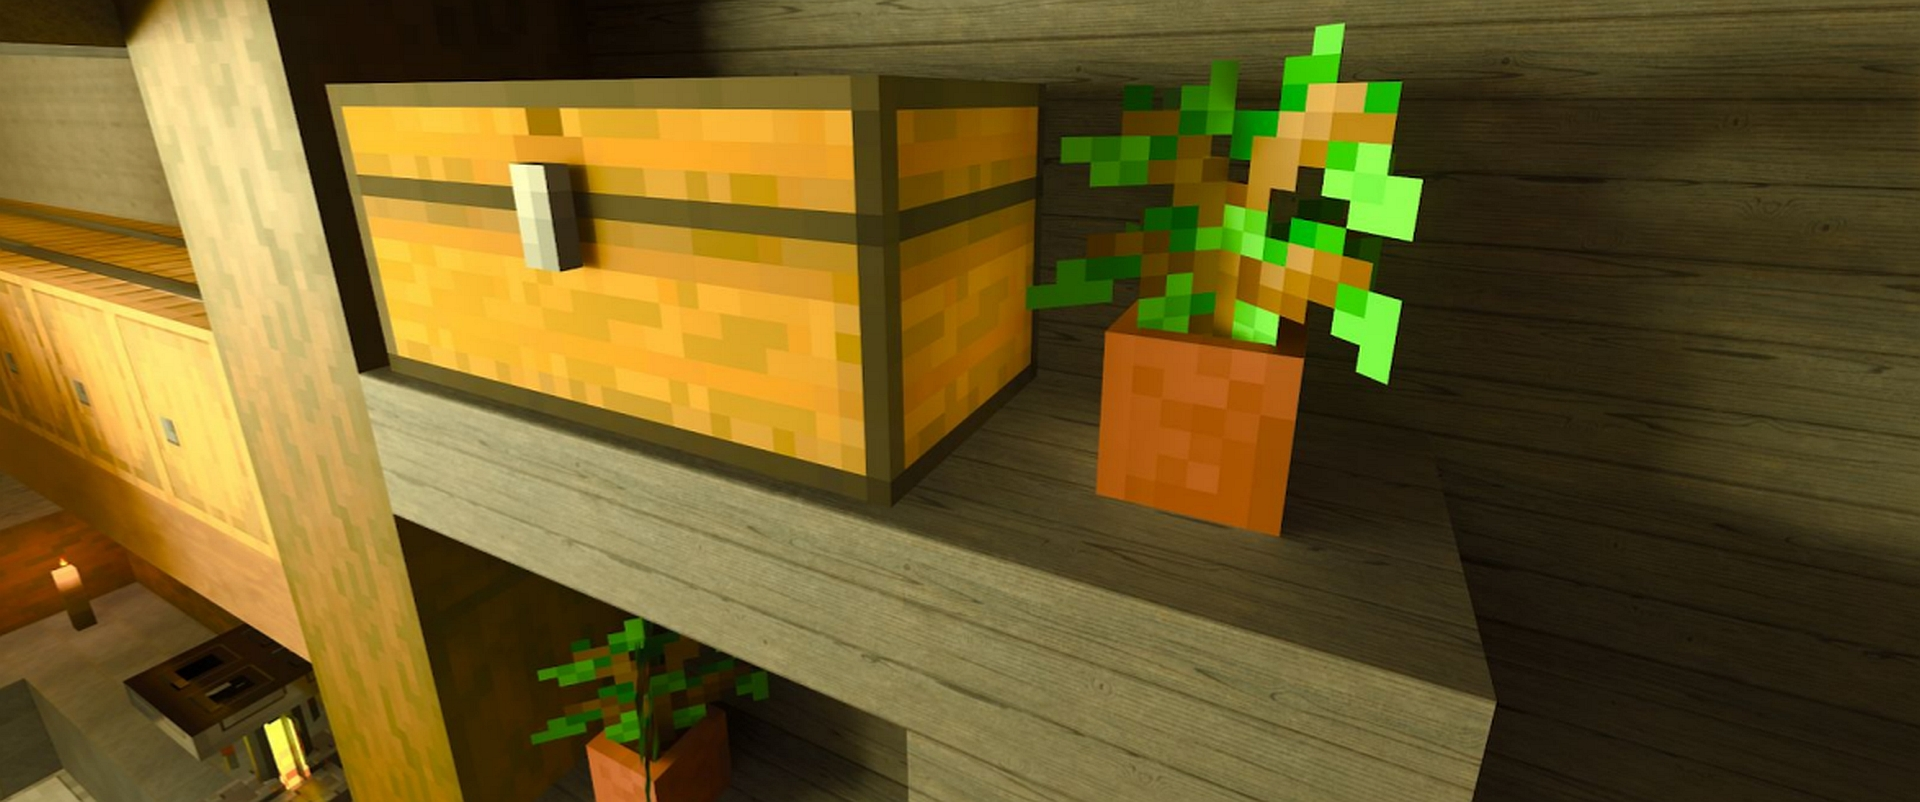
\includegraphics[width=\textwidth]{minecraft.jpg}
      \caption{Graphics from \textit{Minecraft}}\label{fig:minecraft}

      What kinds of lighting and graphics effects do you see in this image?
    \end{figure}
    % By the end of this presentation, we'll have a better understanding of how these graphics are generated
    % We'll also go over some of the math behind it, which will help you build your own graphics scenes
  \end{frame}

  \begin{frame}
    \begin{figure}
      \centering
      \includegraphics[width=\textwidth]{cars.png}
      \caption{Graphics from the movie \textit{Cars}}\label{fig:cars}

      What about this image?
      % global illumination techniques
      % ambient occlusion
      % depth of field
    \end{figure}
    % By the end of this presentation, we'll have a better understanding of how these graphics are generated
    % We'll also go over some of the math behind it, which will help you build your own graphics scenes
  \end{frame}

  \begin{frame}
    \begin{figure}
      \centering
      \includegraphics[width=\textwidth]{lastofuspart2.png}
      \caption{Graphics from \textit{The Last of Us Part II}}\label{tlou2}

      What about this image?
      % subsurface scattering in the skin
      % translucency in the hair
      % realistic light interactions with cloth
    \end{figure}
  \end{frame}




  \begin{frame}
    \frametitle{Physics of Light}
    \begin{itemize}
      \item The Basics of Light
      % Speaker notes: This is a good place to mention that light is a particle, but it's also a wave. We're going to focus on the particle aspect of light.
      % Focusing on the particle aspect of light is important because it allows us to model light as a ray. We'll get to this later.
      % A light particle - a photon - has two key characteristics that are important to us:
      % - it has a wavelength, which determines its colour
      % - it has a direction, which determines where it goes
      \item Reflection of light % we don't need to discuss refraction
      % Speaker notes: Reflection is a very important concept in computer graphics.
      % It's important because it's the basis of a lot of shading techniques that we'll discuss later.
      % We have two types of reflection: diffuse and specular.
      \begin{figure}
        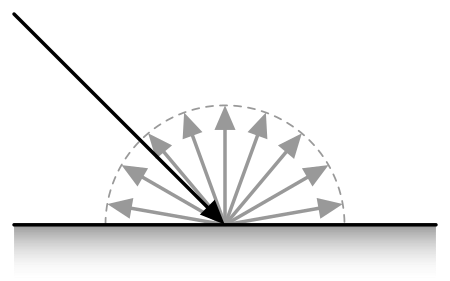
\includegraphics[width=0.4\textwidth]{diffuse}
        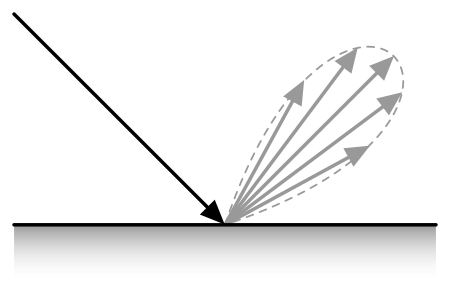
\includegraphics[width=0.4\textwidth]{specular}
        \caption{Diffuse (left) versus Specular reflection (right)}\label{fig:diffuse_specular}
      \end{figure}
      % Diffuse reflection is the reflection of light from a surface that is not smooth.
      % As we can see, the light is scattered in all directions.
      % SHOW LASER DEMO: shine a laser against *any* surface and you'll see that the light is scattered in all directions.
      % Even though a laser is a point light - and we know that in specular reflection, the light is reflected in a single direction - the light is still scattered in all directions.
      % The overall interaction of light on a given surface is a combination of diffuse and specular reflection inherent in the material properties of the surface.
      % the brightest point of reflection off a surface is given by the specular reflection.
      % The rest of the light is scattered in all directions by the diffuse reflection.

    \end{itemize}
  \end{frame}

  \begin{frame}
    \frametitle{Reflection: Mathematically}
    \begin{itemize}
      \item Angle of incidence and angle of reflection
      % Specular reflection, where the light is reflected in a single direction, is determined by the angle of incidence and the angle of reflection.
      % When we have an arbitrary surface, the angle of incidence is the angle between the normal of the surface and the direction of the incoming light.
      % *draw on board* or make a TikZ diagram
      \begin{itemize}
        \item Law of reflection: angle of incidence = angle of reflection

        \[
          \theta_i = \theta_r
        \]
      \end{itemize}
      \item Surface normals: A vector perpendicular to the surface.

      \includegraphics[width = 0.9 \textwidth]{reflection.png}

      \caption{\tiny{Image Credit: Leonid Sigal, CPSC 425 Lecture Slides}}
      % But, if we want to find the normal of a simple surface such as a cube or a sphere, we can use the following formula:

      % make a table with the formula for the normal of a cube and a sphere
      % \begin{table}
      %     \centering
      %     \begin{tabular}{|c|c|}
      %         \hline
      %         \textbf{Surface} & \textbf{Normal} \\
      %         \hline
      %         \hline
      %         \textbf{Cube} & \begin{align*}
      %             \frac{p}{|p|}
      %         \end{align*} \\
      %         \hline
      %         \textbf{Sphere} & \begin{align*}
      %             \frac{p - c}{|p - c|}
      %         \end{align*} \\
      %         \hline
      %     \end{tabular}
      %     \caption{Surface normals}
      % \end{table}

      % where $p$ is the point on the surface and $c$ is the centre of the sphere.

      % So, for example, if I'm on the side of a cube that's facing me, the normal of the surface is going to be pointing towards me.
      % Given we're dividing by the magnitude of the vector, the normal is always going to be a unit vector.
      % And the coordinates of a cube always have one of the coordinates equal to the size of the cube.

      % And for a sphere, the normal is going to be pointing away from the centre of the sphere.

    \end{itemize}
  \end{frame}

  \begin{frame}
    \frametitle{Tracing light through an object}
    Let's start with a point light source interacting with a mirror.

    If I want to trace the light from a light source to a point on a surface, I can do so by first finding the direction of the light.
    This is pretty arbitrary, as point light sources scatter in all directions.
    So, we can just pick one.
    Let's call this our ray.

    \includegraphics[width = \textwidth]{lt1.png}

  \end{frame}

  \begin{frame}
    \frametitle{Tracing light through an object - continued}


    % draw a diagram of a ray from a light source in a random direction
    % \begin{tikzpicture}
    %     % light source is just a sphere at the origin
    %     \draw[fill=black] (0,1) circle (0.1);
    %     % draw a ray pointing in a random direction
    %     \draw[->, thick] (0, 1) -- (1, 0);
    % \end{tikzpicture}

    I then want to follow that ray until it hits a surface.

    \includegraphics[width = \textwidth]{lt2.png}

    % \begin{tikzpicture}
    %     % light source is just a sphere at the origin
    %     \draw[fill=black] (0,1) circle (0.1);
    %     % draw a ray pointing in a random direction
    %     \draw[->, thick] (0, 1) -- (1, 0);
    %     % draw a cube at (1, 0)
    %     \draw[fill=black] (1, 0) cube (1);
    % \end{tikzpicture}

  \end{frame}

  \begin{frame}
    \frametitle{Tracing light through an object - continued}
    Once it hits that surface, I find the normal of the surface at the point of intersection.
    % Again, for a cube or a sphere, this is pretty easy to do.

    % \begin{tikzpicture}
    %     % light source is just a sphere at the origin
    %     \draw[fill=black] (0,1) circle (0.1);
    %     % draw a ray pointing in a random direction
    %     \draw[->, thick] (0, 1) -- (1, 0);
    %     % draw a cube at (1, 0)
    %     \draw[fill=black] (1, 0) cube (1);
    %     % draw the normal of the surface at the point of intersection
    %     \draw[->, thick] (1, 0) -- (1, 1);
    % \end{tikzpicture}

    \includegraphics[width = \textwidth]{lt3.png}

  \end{frame}

  \begin{frame}
    \frametitle{Tracing light through an object - continued}

    I then want to find the angle of incidence between the normal and the ray, and then bounce the ray off the surface according to the law of reflection.

    \includegraphics[width = \textwidth]{lt4.png}

  \end{frame}

  % draw the reflected ray in a different colour
  % \begin{tikzpicture}
  %     % light source is just a sphere at the origin
  %     \draw[fill=black] (0,1) circle (0.1);
  %     % draw a ray pointing in a random direction
  %     \draw[->, thick] (0, 1) -- (1, 0);
  %     % draw a cube at (1, 0)
  %     \draw[fill=black] (1, 0) cube (1);
  %     % draw the normal of the surface at the point of intersection
  %     \draw[->, thick] (1, 0) -- (1, 1);
  %     % draw the reflected ray
  %     \draw[->, thick, color=red] (1, 0) -- (0, 1);
  % \end{tikzpicture}

  \begin{frame}
    \frametitle{Tracing light through an object - continued}

    We can then move on to the next surface - whatever the light is heading towards next - and repeat the process.

    \includegraphics[width = \textwidth]{lt5.png}

    This process of casting a ray from a light source to a surface and determining where it first hits a surface is called ray casting.

  \end{frame}

  \begin{frame}{Where the light ends up}
    \includegraphics[width = 0.8 \textwidth]{lt5.png}
    Once the light hits the camera, we now know the path of the light up until it hits the camera. The object that it was at immediately before will be visible in our scene.

  \end{frame}

  \begin{frame}
    \frametitle{Scene Geometry}

    % If we want to go from tracing a single ray to performing actions on an entire scene of objects, we need to be able to represent the scene in a way that we can easily manipulate.

    % We can do this by representing the scene as a collection of objects, each with a position, a size, and a colour.
    % We also have a floor that these objects are sitting on.

    To view the scene we're looking at today, navigate to the following website:

    \url{https://phas.ubc.ca/~ashtan/}

    \hfill

    From there, go to "WebGL Demonstrations" and click on "Scene Geometry".

    Here, you can view the scene that we've recreated in real life and interact with it.

  \end{frame}

  %     \begin{itemize}
  %         \item Camera Geometry
  %         As you're moving around the scene, you'll notice that the scene is being rendered from a particular point of view: the camera.
  %         The camera is a point in space that is looking at the scene.
  %         It has a given field of view, which is the angle that it can see.
  %         This field of view is represented by the distance between the camera and a plane.
  %         This plane is called the near plane, and it's the closest that the camera can see.

  \begin{frame}
    \frametitle{Shading}
    % We've figured out how to determine which objects are visible to a light source - meaning, what objects - or faces of objects - are lit up by a light source.
    % Now, we need to figure out how to determine the colour of those objects: how they look when they're lit up.

    Say we know where the light source is, where we're viewing the object from, and where the object is in space.

    \hfill

    % Once light hits an object, reflecting that light off of the object and onto other objects is a bit of a complicated process - let's look at that a bit later.

    % So let's think of ways that we can approximate the colour of an object just knowing what we mentioned above.
    How can we approximate the colour of an object, just knowing what we talked about?

  \end{frame}

  \begin{frame}
    \frametitle{A Simple Approach to Shading} % i.e. flat shading

    From where the light source is and the face of the object that's being lit up, we can determine the angle of incidence between the light source and the face of the object.

    A simple approach is to just make the object brighter the smaller the angle of incidence is.
    % This means that if a face is barely visible to the light source, it won't be as bright as a face that's directly facing the light source. % show a diagram of this on the white board

    % If we break up our object into a grid of squares, we can then determine the colour of each square by determining the angle of incidence between the light source and the normal of the square.

    % Of course, we're ignoring so much here - the fact that light is reflected off of the object, the fact that we might have both diffuse and specular reflection, and much more. But this is a good start.

    % We can improve this model by smoothing out the colour of the object by averaging the colour of the squares that are adjacent to each other. % This is called Gouraud shading.

    \begin{figure}
      \centering
      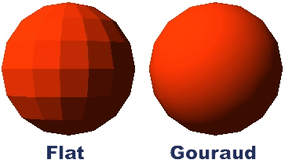
\includegraphics[width=0.4\textwidth]{flatvsgouraud.png}
      \caption{Simple approaches to shading}\label{fig:shading}
      % credits: https://electronics.howstuffworks.com/question484.htm
    \end{figure}

  \end{frame}

  \begin{frame}
    \frametitle{An Equation to Model Light}

    Let's start to build something that we can use to calculate light at a given point.

    \hfill

    It'll be a function, that will be in terms of the angle of the incoming light $(\theta_i, \phi_i)$ and the angle of the camera, i.e. the viewing angle ($\theta_v, \phi_v)$.

    \hfill

    We'll call it the \textbf{Bidirectional Reflection Distribution Function}, or \textbf{BRDF} for short.

  \end{frame}

  \begin{frame}
    \frametitle{Building up the BRD} % i.e. phong shading

    We know from our real-life experiences that light is also reflected off of other objects: If we go outside, even if the sun isn't directly shining on us, we can still see other things around us.
    Let's call that "ambient light".

    \hfill

    Ambient light can be approximated in our BRDF with a simple constant representing the amount of ambient light in the scene:

    $$\boldsymbol{B R D F}() = \alpha_{ambient}$$

  \end{frame}

  \begin{frame}{Building up the BRDF}
    We talked about diffuse reflection before. We know it only depends on the incoming angle $\theta_i$ - this is called \textbf{Lambert's Cosine Law}:
    \begin{figure}
      \centering
      \includegraphics[width=0.9 \textwidth]{lambert.png}
    \end{figure}

    $$\boldsymbol{B R D F}\left(\theta_i \right) = \alpha_{ambient} + \alpha_{diffuse} \cos(\theta_i)$$

  \end{frame}

  \begin{frame}
    \frametitle{A Better Approximation}

    Lastly, we just need to add a term that depends on the viewing angle as well to determine the specular component.

    \hfill

    It'll be brighter when the viewing angle is close to the reflected angle, so we have the following:

    $$\boldsymbol{B R D F}\left(\theta_i, \theta_v \right) = \alpha_{ambient} + \alpha_{diffuse} \cos(\theta_i) + \alpha_{specular} \cos^{\beta}(\theta_v)$$

    Here, $\beta$ is the shininess of the object.

    \hfill

    This is for two dimensions. In three dimensions the $\cos()$ terms are replaced by dot products with the normal vector, giving dependence on $\phi$ angles also.

  \end{frame}


  \begin{frame}
    \frametitle{A Better Approximation}

    So we can add up all of these components - ambient, diffuse, and specular - to determine the overall shading of the object.
    This is then done for all the faces of the object, and all objects in the scene.

    \begin{figure}
      \centering
      \includegraphics[width=0.8\textwidth]{phong-shading.png}\label{fig:phong-shading}
    \end{figure}

    You can see what this looks like in our WebGL demo by navigating to the same website as before, clicking on WebGL demos, and click the "Phong Shading" button.

    \url{https://phas.ubc.ca/~ashtan/}

  \end{frame}

  \begin{frame}{Phong Shading in \textit{Half-Life 2}}

    \begin{figure}
      \centering
      \includegraphics[width = \textwidth]{halflife2}
      \caption{Phong shading used in \textit{Half-Life 2}. Note the reflection of the light source on the rocks.}
      \label{fig:hl2}
    \end{figure}

  \end{frame}

  % \begin{frame}
  %     \frametitle{A Caveat}

  %     \begin{itemize}

  %      % I've mentioned a few different names for the types of shading we've discussed so far. These names aren't really important - you don't have to memorize them, but I want to mention them because they're used in the literature if you want to learn more about these topics.
  %     \item These names aren't important! Just provided if you want to learn more.

  %     % For reference, Phong shading is the standard shading model that's used widely in computer graphics, especially in video games as it can be done in real time (as you can see in the demo).
  %     \item Phong shading: The standard for video games and other real-time graphics.

  %     \end{itemize}
  % \end{frame}

  \begin{frame}{What's missing in our BRDF?}

    We now know how to determine the shading of an object given the position of the light source and the camera.

    But we haven't actually done anything \textit{more} with the light rays that are being reflected off of the initial object.

    \begin{figure}
      \centering
      \includegraphics[width = 0.8 \textwidth]{lt6.png}
    \end{figure}

    So, we need to figure out how to follow the reflected light throughout the scene until it hits our camera.

  \end{frame}

  % \begin{frame}
  %   \frametitle{Tracing Rays}



  % From what we can see in the Phong shading demo, there aren't any shadows, and the scene doesn't look very realistic.
  % The metallic objects aren't reflecting any of the light that hits them, and it just looks like a gray surface with some texture on it.



  % \end{frame}

  \begin{frame}
    \frametitle{A Naive Approach}

    Intuitively, light travels from the light source, interacts with a scene, and then travels either to the camera, gets fully absorbed, or exits the scene.

    So we can build an algorithm that does exactly that.

  \end{frame}

  \begin{frame}[fragile]

    \footnotesize            \begin{lstlisting}[label={lst:pseudocode-raytrace}]
for each light source:
    for each angle:
        cast a ray from light source at angle
        while the ray hasn't hit anything:
            if ray hits an object:
                determine the colour of obj
                add obj color to light source color
                Bounce ray off object and continue
            if ray hits camera:
                add ray color to pixel in camera frame
            If ray exits scene: break
    \end{lstlisting}

  \end{frame}

  \begin{frame}
    \frametitle{In practice - A simple model}

    % Just as we mentioned before that the most simple objects to render are spheres, the most simple scene to render is a scene with only a sphere.
    % So let's take a look at what that looks like.

    % We've built up the scene using the algorithm we discussed above.
    Using the algorithm we just discussed, let's render a sphere. Just one object.

    \hfill


    Play around with the demo by clicking on "Ray Tracing - Sphere".

    \hfill

    (website: \url{https://phas.ubc.ca/~ashtan/})

    % Moving the mouse or your finger will move the light source around the scene.

    % (Demo Credits: Sushindhran Harikrishnan, \url{https://medium.com/neosavvy-labs/webgl-2-0-ray-tracing-34866baca7c1})

  \end{frame}

  \begin{frame}
    \frametitle{Real Life Demonstration}

    Let's see what a ray trace would look like in real life using the same scene as before, this time using the real-life scene as a reference.
    We'll see why we're using our real life demonstration to trace the rays to begin with in a moment.

    % this is the cubes demo

    \begin{itemize}
      \item Starting with a single light ray (laser)
      % We see that the light is reflected off of the objects, using both diffuse and specular reflection.
      % the light rays travel until they either hit the camera, get absorbed, or exit the scene.
      \item Point light source (flashlight)
      % the scene is fully lit up - we have tons of light rays bouncing around the scene.
      % this, of course, generates an accurate depiction of the scene (but it's real life, so of course it's accurate)
    \end{itemize}

  \end{frame}

  \begin{frame}

    How many rays of light do you think there are in this room?

  \end{frame}

  \begin{frame}

    % answer to the previous question
    A light bulb (of around 100 watts) emits $10^{20}$ photons per second (and that's \textit{one light source}).

    % Regardless of if the actual number is higher or lower, we can see that this is a lot of rays of light.
    \hfill

    And we have to trace the path for \textbf{every} ray of light?
    It's an understatement to say that this is a lot of computation.

    \hfill

    We need to find a way to reduce the number of rays of light that we have to trace.

    First, let's change our perspective on this problem. (pun intended)

  \end{frame}

  \begin{frame}
    \frametitle{A change in perspective}

    \begin{itemize}
      \item We know light will travel in a given path from the light source to the camera.
      \item We also know that light will travel in a given path from the camera to the light source.
      \item These paths are the same!
    \end{itemize}

    \hfill

    When we have light exiting the scene without hitting the camera, it's a waste of computational power to bother calculating the path of that ray.

    % And, when we consider the size of the camera frame in comparison to the size of the scene, we can see that the probability of a ray of light exiting the scene without hitting the camera is very high.

    % So, we can draw the rays starting from the camera and going outward to the scene.

  \end{frame}

  \begin{frame}
    \frametitle{Outwards from the camera}

    How do we do this?

    We first need to take a look at how we're representing our camera.
    This is dependent on whether we're looking for accurate perspective, or if we're looking to analyze a selection of a scene.

    % If we're looking for accurate perspective, we choose a pinhole camera. The field of view of the camera is given by how close the camera is to the viewing plane (the viewing plane is exactly what we see on the screen).

    % If the camera is further away, we minimize the depth of field. On an infinite distance the depth of field is zero and we have an orthographic camera where the projection view is parallel to the viewing plane.

    \begin{figure}
      \centering
      \includegraphics[width=0.5\textwidth]{pinhole-camera.png}
      \caption{Different camera models and their field of view}\label{fig:camera-models}
    \end{figure}

  \end{frame}

  \begin{frame}
    \frametitle{Choosing the angle of the ray}

    If we draw a line from the pinhole to the pixel we're interested in, it forms the beginning of the ray that's already in the direction we want it to go.

    \begin{figure}
      \centering
      \includegraphics[width=0.4\textwidth]{coordinates-camera.png}
      \caption{Camera local coordinate system with the "screen" in the Z=0 plane}\label{fig:camera-coordinates}
    \end{figure}

    % So if we continue these rays outward into the scene, we can determine what they hit, and therefore what objects are visible directly to the viewer.

    % And \textbf{all} of the rays that we trace now all hit the camera, because that's where we started from. We're on our way to a vastly increased efficiency.

  \end{frame}

  \begin{frame}
    \frametitle{Ray tracing our scene: Putting it into perspective}

    % \begin{figure}
    %   \centering
    %   \includegraphics[width=0.5\textwidth]{ray-tracing-scene.png}
    %   \caption{Ray tracing our scene}\label{fig:ray-tracing-scene}
    % \end{figure}

    % this is the same scene as before and as in our real life demonstration
    % point out the shadows to the students

    Check out a rendered video of this scene on the Demos page, under "Ray Tracing - Scene".

  \end{frame}

  \begin{frame}
    \frametitle{We don't actually trace $10^{20}$ rays}

    We can't actually trace $10^{20}$ rays, of course.
    That'd be crazy.

    \hfill

    The actual number is comparatively small.

    \hfill

    When we choose, say, a 1920x1080 camera frame, we have 2,073,600 pixels - and therefore 2,073,600 rays to trace.
    We can also choose to cast multiple rays per pixel, which will increase the accuracy of the scene.

    % a 1920x1080 camera frame was exactly what was chosen for our ray tracing demo
    % Put it into perspective for students - this scene has 172 frames and each scene took around a minute to render. That's just under 3 hours of rendering time.
    % compare that to real time rendering using Phong shading, which took a few seconds to render the same scene.

  \end{frame}

  \begin{frame}
    \frametitle{We're almost there! What's didn't we cover today?}

    \begin{itemize}
      \item Multiple reflections coming from the same point
      \begin{itemize}
        \item e.g.\ a light ray partially reflecting off of a surface and partially being transmitted through (see Figure \autoref{fig:caustics})

        \begin{figure}
          \centering
          \includegraphics[width=0.3\textwidth]{caustics.png}
          \caption{Caustics produced by a water glass}
          \label{fig:caustics}
        \end{figure}

        \item Recursive ray tracing is a solution to this problem

      \end{itemize}

    \end{itemize}

  \end{frame}

  \begin{frame}
    \frametitle{We're almost there! What's didn't we cover today?}

    \begin{itemize}

      \item De-noising the image

      \begin{itemize}
        \item One ray per image leads to a lot of noise caused by jagged edges
        \item there are a few de-noising techniques that can be used to reduce the noise
      \end{itemize}

      \item Creating textures

      \begin{itemize}
        \item This is a complicated computer graphics topic!
        You could have a whole course on geometric modelling.
      \end{itemize}

    \end{itemize}

  \end{frame}

  \begin{frame}{What benefits does ray tracing have?}

    \begin{itemize}
      \item It's a very accurate way of rendering a scene - it can be used to create photorealistic images
      \item It allows us to model complex phenomena, such as soft shadows, volume rendering, and caustics
      \item It's a very flexible rendering technique % - it can be used to render any scene, regardless of the complexity of the scene
    \end{itemize}

    But we have to ask - Are these benefits worth the drastically increased computational cost?
  \end{frame}

\end{document}
